\documentclass[11pt,a4paper]{article}
    \usepackage[margin=2.5cm]{geometry}
    \usepackage{enumitem}
    \usepackage{hyperref}
    \usepackage{tikz}
    \usetikzlibrary{arrows.meta,positioning,shapes.geometric}
    \title{Python Primer}
    \author{CBBL Tools}
    \date{\today}

    \tikzset{
      methodbox/.style={
        rounded corners=6pt,
        draw=blue!50!black,
        line width=0.9pt,
        fill=blue!6,
        minimum width=13cm,
        text width=11.8cm,
        align=left,
        inner sep=8pt
      }
    }

    \begin{document}
    \maketitle

    \section*{Scope}
    This folder is an introductory teaching collection for basic Python syntax, file handling, plotting, modules, and simple automation tasks.

    \section*{Material in this folder}
    \begin{itemize}[leftmargin=*]
\item \texttt{BasicPythonIntro.ipynb}
\item \texttt{DuplicatedFiles.ipynb}
\item \texttt{Operators.ipynb}
\item \texttt{ReadPDFfiles.ipynb}
\item \texttt{Remove empty directories.ipynb}
\item \texttt{Simple\_matplotlib.ipynb}
\item \texttt{extractIntAct.ipynb}
\item \texttt{moduleExample.ipynb}
\item \texttt{map.py}
\item \texttt{module1.py}
    \end{itemize}

    \section*{Method summary}
    \begin{itemize}[leftmargin=*]
\item \textbf{Core language basics}. The notebooks cover operators, modules, introductory syntax, and small self-contained examples.
\item \textbf{Filesystem operations}. Several notebooks demonstrate how to detect duplicated files or remove empty directories.
\item \textbf{Input-output and external data}. The materials include simple PDF handling, file downloads, and a world-map plotting example.
\item \textbf{Reusable module construction}. The example module defines simple functions and shows how import-based code reuse works.
    \end{itemize}

    \section*{Method scheme}
    Figure~\ref{fig:summary} is drawn directly in LaTeX with TikZ. It is a compact conceptual map of the main workflows discussed in this folder.

    \begin{figure}[ht]
    \centering
    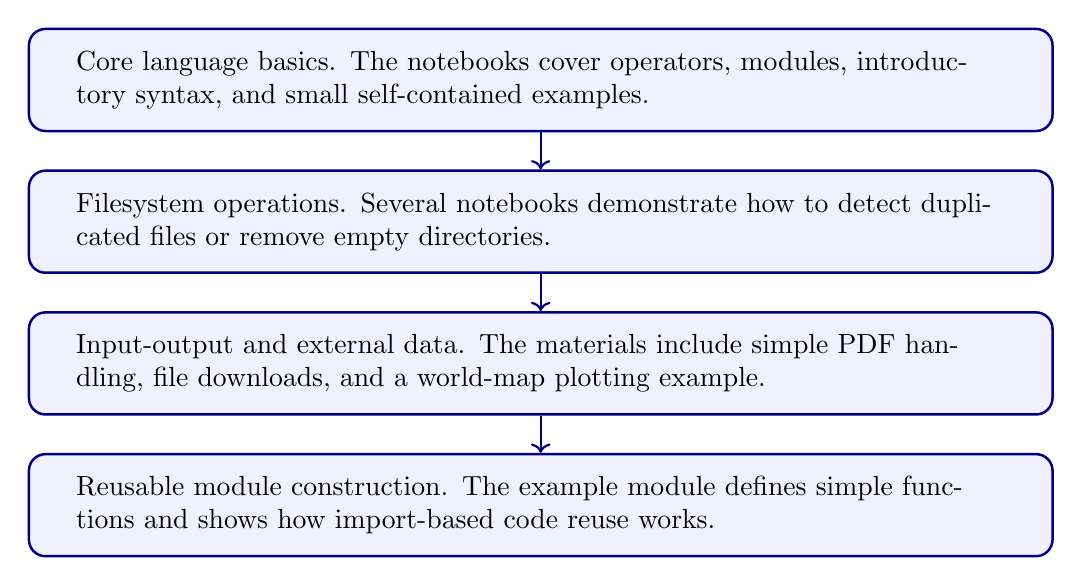
\begin{tikzpicture}[x=1cm,y=1cm]
    \node[methodbox] (m0) at (0,0.0) {Core language basics. The notebooks cover operators, modules, introductory syntax, and small self-contained examples.};
    \node[methodbox] (m1) at (0,-1.8) {Filesystem operations. Several notebooks demonstrate how to detect duplicated files or remove empty directories.};
    \node[methodbox] (m2) at (0,-3.6) {Input-output and external data. The materials include simple PDF handling, file downloads, and a world-map plotting example.};
    \node[methodbox] (m3) at (0,-5.4) {Reusable module construction. The example module defines simple functions and shows how import-based code reuse works.};
    \draw[->, thick, color=blue!50!black] (m0.south) -- (m1.north);
    \draw[->, thick, color=blue!50!black] (m1.south) -- (m2.north);
    \draw[->, thick, color=blue!50!black] (m2.south) -- (m3.north);
    \end{tikzpicture}
    \caption{Conceptual scheme for the methods in the pythonPrimer folder.}
    \label{fig:summary}
    \end{figure}

    \end{document}
